\chapter{Sprays}\label{chap1:chap1}

Throughout \pageoriginale this chapter $M$ stands for a manifold and
$(U,r)$ for a typical chart of it.

\section{Definition.}

\begin{figure}[H]
\centering
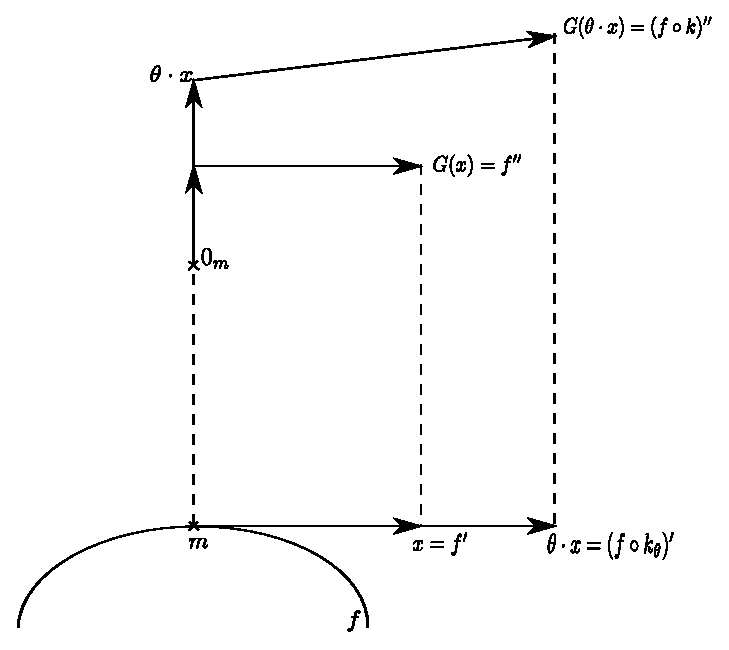
\includegraphics[scale=.7]{chap1-fig1.eps}
\end{figure}


\quad Our aim now is to define a ``geodesic'' so as to generalise a curve
which is intuitively the shortest distance between two points on it,
which are sufficiently close. Such a definition must have the
following natural properties:
\begin{enumerate}
\renewcommand{\labelenumi}{\rm\theenumi)}
\item A geodesic curve is uniquely determined by its initial position
  and speed.

\item A change of parameter by a homothesy or a translation 
  leaves \pageoriginale it
  a geodesic. So the family of geodesics determines a family of curves
  on $T(M)$ one passing through each point $x$ of $T(M)$. Associating
  to each point $x$ of $T(M)$ the tangent vector at $x$ of the unique
  curve of the family passing through $x$ we get a map (set theoretic)
  $:G:T(M)\to T(T(M))$.
\end{enumerate}

We have by the very definition and from \ref{chap0:0.5.9} together with
\ref{chap0:0.4.20}
\begin{equation*}
f''=G\circ f'\tag{1}\label{chap1:eq1}
\end{equation*}
and
\begin{equation*}
p'\circ G=p^{T}\circ G=\id_{T(M)}\tag{2}\label{chap1:eq2}
\end{equation*}
for any geodesic curve $f$. Further we have $f\circ k_{\theta}$ is a
geodesic curve, and hence
\begin{equation*}
(f\circ k_{\theta})''=G\circ (f\circ k_{\theta})'.\tag{3}\label{chap1:eq3}
\end{equation*}

But we have for $x=f'(0)$ and by \ref{chap0:0.5.11}:
$$
(f\circ k_{\theta})'=\theta f'(0)=\theta\cdot x
$$
and
$$
(f\circ k_{\theta})''(0)=\theta\cdot (h^{T}_{\theta}\circ
f''(0))=\theta\cdot (h^{T}_{\theta}\circ G(x))
$$
and so
\begin{equation*}
G\circ h_{\theta}=\theta(h^{T}_{\theta}\circ G)\tag{4}\label{chap1:eq4}
\end{equation*}

Thus from the concept of a geodesic we are led to a $G$ with the
properties \eqref{chap1:eq2} and \eqref{chap1:eq4}. Keeping this in
mind we reverse the process and \pageoriginale first define a spray and
then a geodesic as its integral curve.

\setcounter{definition}{0}

\subsection{}\label{chap1:1.1.1}

%\setcounter{section}{1}
\begin{defi*}
A {\em spray} $G$ on $M$ is an element of $\mathscr{C}(T(M))$ such
that
\begin{itemize}
\item[\rm 1)] $p^{T}\circ G=\id_{T(M)}$ and

\item[\rm 2)] $G\circ h_{\theta}=\theta(h^{T}_{\theta}\circ G) \, \forall
  \theta\in \mathbb{R}$
\end{itemize}
\end{defi*}

\setcounter{subsection}{1}

\subsection{}\label{chap1:1.1.2}

\begin{note*}
From 2) it follows that
$$
G(0_{m})=0\,\forall m\in M
$$
Generally we denote a spray by $G$.
\end{note*}

\setcounter{subsection}{2}
\subsection{}\label{chap1:1.1.3}
If $N$ is an open sub manifold of $M$, $G$ induces a spray on $N$ and
{\em we denote it by} $N_{G}$.

\section{Geodesics}\label{chap1:sec2}

Now we define a geodesic curve.


\subsection{}\label{chap1:1.2.1}

\begin{defi*}
A {\em geodesic} of $M$ relative to a spray $G$ is a curve $f$ in $M$
such that $f'$ is an integral of $G$, i.e. $f$ is such that
$$
f''=G\circ f'.
$$
\end{defi*}

\subsection{}\label{chap1:1.2.2}

\begin{remark*}
If $f:[0,1]\to M$ is a geodesic, then the curve $g:[0,1]\to M$ defined
by $g(t)=f(1-t)$ is a geodesic.
\end{remark*}

When no confusion is possible, we shall speak simply of a geodesic and
omit the reference to the spray.

\subsection{}\label{chap1:1.2.3}

\begin{prop*}
$f$ is a geodesic if and only if there exists an integral $g$ of $G$
  such that
$$
f=p\circ g.
$$
\end{prop*}

\begin{proof}
If \pageoriginale $g$ is an integral of $G$ then $g'=G\circ g$ and then
if $f=p\circ g$, we have
$$
f'=p^{T}\circ g=p^{T}\circ G\circ g=g\quad\text{since}\quad p^{T}\circ
G=\id_{T(M)}. 
$$
Hence $f$ is a geodesic. For the other part, if $f$ is a geodesic we
can take $g=f'$ for the integral of $G$.
\end{proof}

\setcounter{subsection}{3}

\subsection{}\label{chap1:1.2.4}

\begin{remarks*}
From (\ref{chap0:0.6.2}) one knows that given $x\in T(M)$ there is, locally,
a geodesic $f$ of $M$ such that $f'(0)=x$, and that it is unique. 
\end{remarks*}

\setcounter{subsection}{4}

\subsection{}\label{chap1:1.2.5}
From the fact that $G(0_{m})=0$ we see that $\forall m\in M$
$f(\mathbb{R})=m$ is a geodesic, called the {\em trivial geodesic} at
$m$. 


\subsection{}\label{chap1:1.2.6}

\begin{prop*}
If $f\in D(I,M)$ is a geodesic so are 
\begin{gather*}
f\circ \tau_{a}\in D(\tau^{-1}_{a}(I), M)\quad\text{and}\\
f\circ k_{\theta}\in D(k^{-1}_{\theta}(I),M)\forall a\in
\mathbb{R},\forall \theta\in \mathbb{R}, \theta\neq 0.
\end{gather*}
\end{prop*}

This proposition is a direct consequence of the definitions.

\subsection{}\label{chap1:1.2.7}


\begin{coro*}
For $x\in T(M)$, $\theta\in \mathbb{R}$ and $t\in \mathbb{R}$ we have
$$
\gamma(t,\theta x)=\theta\cdot \gamma(t\theta,x),
$$
i.e. whenever one of these terms is defined so is the other and the
equality holds.
\end{coro*}

\begin{proof}
Let $f$ be the geodesic with $f'(0)=x$ and let $g=f\circ
k_{\theta}$. Then $g$ is the geodesic with $g'(0)=\theta\cdot x$ and
we have by the definition \pageoriginale of $\gamma$
$$
f'(t)=\gamma(t,x)
$$
and
$$
g'(t)=\gamma(t,\theta x)
$$
But then
$$
\gamma(t,\theta x)=g'(t)=\theta\cdot f'(\theta\cdot t)=\theta\cdot
\gamma(\theta\cdot t,x).
$$
\end{proof}

\subsection{}\label{chap1:1.2.8}

\begin{coro*}
For $x\in T(M)$ and $\theta\in\mathbb{R}$ and $\neq 0$, we have
\begin{align*}
t^{+}(\theta\cdot x) &= \theta^{-1}(t^{+}(x))\\
\text{and}\qquad t^{-}(\theta\cdot x) &= \theta^{-1}(t^{-}(x))
\end{align*}
\end{coro*}

\begin{proof}
If $f$ is the geodesic of $M$ on $]t^{-}(x)$, $t^{+}(x)[$ then
$$
f\circ k_{\theta}\quad\text{on}\quad ]\theta^{-1}t^{-}(x), \theta^{-1}t^{+}(x)[
$$
is a geodesic of $M$ with speed $\theta\cdot x$. Hence by the
definitions of $t^{-}$ and $t^{+}$ (see \ref{chap0:0.6.4})
\begin{align*}
& t^{-}(\theta\cdot x)\leq \theta^{-1}\cdot t^{-}(x)\\
\text{and}\qquad & t^{+}(\theta\cdot x)\geq \theta^{-1}\cdot t^{+}(x).
\end{align*}
The other inequalities follow if we interchange the roles of $f$ and
$f\circ k_{\theta}$.
\end{proof}

\section{Expressions for the spray in local coordinates}\label{chap1:sec3}

Let $(U,r)$ be a chart and let
$x{\displaystyle{\mathop{=}_{\cup}}}(a,b)$,
$G(x){\displaystyle{\mathop{=}_{\cup}}}(a,b,c,d)$ (see \ref{chap0:sec4})

Then from the condition 1)~for a spray and from \eqref{chap0:0.4.6} we have
$b=c$. Setting $d=\psi(a,b)$ we have
\begin{align*}
& \psi\in D((r(U)\times R^{d}),R^{d}),\quad\text{and}\\
& G(\theta\cdot x)=(a,\theta b,\theta b,\psi(a,\theta b)),\\
& h^{T}_{\theta}(G(x))=(a,\theta b,b,\theta\cdot\psi(a,b)),
\end{align*}
and\pageoriginale
$$
\theta h^{T}_{\theta}(G(x))=(a,\theta b,\theta b,\theta^{2}\cdot \psi(a,b)).
$$

Now from the second condition for a spray we get
$$
G(\theta\cdot x)=\theta(h^{T}_{\theta}(G(x)))
$$
and hence
\begin{equation*}
\psi(a, \theta b)=\theta^{2}\cdot \psi(a,b)\,\forall \theta\in
\mathbb{R}\tag{1.3.1}\label{chap1:1.3.1}
\end{equation*}

Using Euler's theorem on homogeneous functions we see that $\psi$ is,
for a fixed $a$, $a$ quadratic form in $b$ so that
\begin{equation*}
\psi(a,b)=(D^{2}\psi_{a})(b\cdot b)\tag{1.3.2}\label{chap1:1.3.2}
\end{equation*}
with $D^{2}\psi$ symmetric. Hence we have the following:


\setcounter{subsection}{2}
\subsection{}\label{chap1:1.3.3}


\begin{prop*}
If $G$ is a spray then there exists, locally, a unique $\delta \in
D(r(U)\times\mathbb{R}^{d}\times \mathbb{R}^{d},\mathbb{R})$ such
that, for $a\in r(U)$, its restriction to $\{a\}\times
\mathbb{R}^{d}\times \mathbb{R}^{d}$ is bilinear, symmetric and
$$
\psi(a,b)=\delta(a,b,b).
$$
\end{prop*}

\setcounter{subsection}{3}
\subsection{}\label{chap1:1.3.4}

{\em Setting}
$\Gamma^{j}_{ik}(a)=-\mathscr{U}^{j}(\delta(a,e_{i},e_{k}))$ for $a\in
r(U)$, we have
$$
\Gamma^{j}_{ik}\in F(r(U)).
$$

Let $f\in D(I,M)$ be a geodesic and let $a=r\circ (f|U)$, be its image
in $r(U)$, then we have
\begin{align*}
& f'(t)\mathop{=}_{\cup}(a(t),\frac{da(t)}{\dt})\\
\text{and}\qquad & f''(t)\mathop{=}_{\cup}(a(t),\frac{da(t)}{\dt}, \frac{da(t)}{\dt},\frac{d^{2}a(t)}{\dt^{2}}).
\end{align*}

So if we write
$$
a(t)=\sum x^{i}(t)e_{i}
$$
then we see that $f$ is a geodesic if and only if 
\begin{equation*}
\frac{d^{2}x^{j}}{\dt^{2}}+\sum_{i,k}\Gamma^{j}_{ik}\frac{dx^{i}}{\dt}\cdot
\frac{dx^{k}}{\dt}=0\forall j.\tag{1.3.5}\label{chap1:1.3.5}
\end{equation*}\pageoriginale

\section{The exponential map}\label{chap1:sec4}

Let us consider $G$ and its flow. Setting
\begin{equation*}\label{chap1:1.4.1}
\Omega=(t^{+})^{-1}(]1, +\infty[)\quad \text{(see \ref{chap0:sec6}a)} \tag{1.4.1}
\end{equation*}
we see, since $t^{+}$ is lower semi continuous, that $\Omega$ is open
in $T(M)$. For every $m\in M$, $0_{m}$ the zero vector at $m$ clearly
belongs to $\Omega$. Hence a neighbourhood of $0_{m}$ is in $\Omega$.

\setcounter{subsection}{1}
\subsection{}\label{chap1:1.4.2}

If $N$ is an open subset of $M$ then by \ref{chap1:1.1.3} there is a
natural spray $N_{G}$ on $N$ and we can define $t^{+}_{N_{G}}$ and
$t^{-}_{N_{G}}$ and $\Omega$ relative to $N_{G}$ and $N$. We denote
this open subset by $N_{\Omega}$. We identify $T(N)$ with an open
sub manifold of $T(M)$ and then, clearly $N_{\Omega}\subset \Omega\cap
T(N)$. Now let $x$ be in $\Omega\cap T(M)$. Then by (0.6.a) it follows
that $x$ belongs to $N_{\Omega}$ if the image of $]0$, $1[$ under
    $p\circ \gamma(t,G(x))$ is in $N$.

\setcounter{subsection}{2}
\subsection{}\label{chap1:1.4.3}

\begin{defi*}
The map $p\circ \gamma_{1}$ from $\Omega$ into $M$ {\em is called the
  exponential map (for the spray $G$) of $T(M)$ and is denoted} by exp.
\end{defi*}

\setcounter{subsection}{3}
\subsection{}\label{chap1:1.4.4}

\begin{note*}
$\exp\in D(\Omega,M)$ because $p$, $\gamma$ are differentiable. {\em
    We denote the restriction of $\exp$} to $T_{m}(M)\cap \Omega$ {\em
    by} $\exp_{m}$.
\end{note*}

\subsection{}\label{chap1:1.4.5}

\begin{lemma*}
For $x$ in $\Omega$ the map 
$$
S:t\to \exp (tx)
$$
defined for sufficiently small $t$ is a geodesic of $M$ and
$S'(0)=x$. In particular $\exp(x)$ is the point $S(1)$ of this geodesic.
\end{lemma*}

\begin{proof}
We have 
\begin{align*}
S(t) &= p\circ \gamma_{1}(tx)=p\circ\gamma(1,tx)\\
 &= p(t,\gamma(t,x))\quad\text{by}\quad \text{(\ref{chap1:1.2.7})}\\
 &= p(\gamma(t,x))
\end{align*}
Hence \pageoriginale $S$ is a geodesic by (\ref{chap1:1.2.3}). The fact that $S'(0)=x$
follows from the definition of $\gamma$.
\end{proof}

\setcounter{subsection}{5}
\subsection{}\label{chap1:1.4.6}
We have
\[
\xymatrix@C=2.5cm@R=1.5cm{
T_{0_{m}}(T_{m}(M))\ar[r]^{\exp^{T}_{m}}\ar[d]_{\zeta} & T_{m}(M)\\
T_{m}(M)\ar[ur]_{\id_{T_{m}(M)}} & 
}
\]

\begin{proof}
For $x$ in $T_{m}(M)$ and $\theta\in\mathbb{R}$ set $\mathscr{U}$
with:
$$
\mathscr{U}(\theta)=\theta\cdot x
$$
so that
$$
\zeta_{0_{m}}(\mathscr{U}'(0))=x.
$$

Now we have
$$
(\exp^{T}\circ\zeta^{-1}_{0_{m}})(x)=\exp^{T}(\mathscr{U}'(0))=(\exp
\circ \mathscr{U})'(0)=S'(0).
$$
and by the preceding lemma we have
$$
S'(0)=x.
$$
\end{proof}

\subsection{}\label{chap1:1.4.7}

Hence it follows by the inverse function theorem that $\exp$ is a
diffeomorphism \pageoriginale between suitable neighbourhoods of
$0_{m}\in T_{m}(M)$ and $m$ in $M$.

\subsection{}\label{chap1:1.4.8}


\begin{coro*}
The map $(p,\exp)$ of $\Omega$ into $M\times M$ has maximal rank at
$0_{m}$ for every $m$ in $M$.
\end{coro*}

\begin{proof}
Since the dimensions of $\Omega$ and $M\times M$ are the same it is
enough to show that the map $(p,\exp)^{T}$ is injective. Now let $z\in
T_{0_{m}}(T(M))$ be such that
$$
(p,\exp.)^{T}(z)=0.
$$
Then since
\begin{equation*}
p^{T}(z)=0\text{ we have } z\in V_{0_{m}}.\tag{1}\label{chap1:sec4-eq1}
\end{equation*}
By the previous proposition we have
\begin{equation*}
\exp^{T}(z)=\zeta(z)\text{ and hence } \zeta(z)=0.\tag{2}\label{chap1:sec4-eq2}
\end{equation*}

The corollary follows from \eqref{chap1:sec4-eq1} and \eqref{chap1:sec4-eq2}.
\end{proof}

